% Nejprve uvedeme tridu dokumentu s volbami
\documentclass[czech,bachelor]{diploma}

% .................................................................... %
% ...................... ZAKLADNI BALICKY MAKER ...................... %

% Dalsi doplnujici baliky maker
\usepackage[autostyle=true,czech=quotes]{csquotes} % korektni sazba uvozovek, podpora pro balik biblatex
\usepackage[backend=bibtex, style=numeric, alldates=iso]{biblatex} % bibliografie
\usepackage{dcolumn} % sloupce tabulky s ciselnymi hodnotami
\usepackage{subfig} % makra pro "podobrazky" a "podtabulky"
\usepackage[cpp]{diplomalst}
\usepackage{listings}
\usepackage{color} %red, green, blue, yellow, cyan, magenta, black, white
\usepackage{fixltx2e}
\usepackage{hyperref}
\usepackage[a4paper,pagesize]{typearea}
\usepackage{float}
\usepackage{amsmath}
\usepackage{setspace}
\usepackage{multirow}

% .................................................................... %
% ...................... PRIDAVNE BALICKY MAKER ...................... %

\usepackage{fancyhdr}
\usepackage{lastpage}
\usepackage{geometry}
\usepackage{graphicx}
\usepackage{epstopdf}
\usepackage[shortlabels]{enumitem}

\usepackage{pifont} %more styles for bullets
\usepackage{wrapfig}
\usepackage{lscape}
\usepackage{rotating}
\usepackage{adjustbox}


% .................................................................... %
% ..................... PRIDANI BIBLATEX SOUBORU ..................... %

\addbibresource{biblatex.bib}
\addbibresource{coffee.bib}

%\bibliography{biblatex-examples}


% .................................................................... %
% ..................... NASTAVENI PRO MATLAB KODY .................... %

\definecolor{mygreen}{RGB}{28,172,0} % color values Red, Green, Blue
\definecolor{mylilas}{RGB}{170,55,241}
\lstset{language=Matlab,%
    %basicstyle=\color{red},
    breaklines=true,%
    morekeywords={matlab2tikz},
    keywordstyle=\color{blue},%
    morekeywords=[2]{1}, keywordstyle=[2]{\color{black}},
    identifierstyle=\color{black},%
    stringstyle=\color{mylilas},
    commentstyle=\color{mygreen},%
    showstringspaces=false,%without this there will be a symbol in the places where there is a space
    numbers=left,%
    numberstyle={\tiny \color{black}},% size of the numbers
    numbersep=9pt, % this defines how far the numbers are from the text
    emph=[1]{for,end,break},emphstyle=[1]\color{red}, %some words to emphasise
    %emph=[2]{word1,word2}, emphstyle=[2]{style},    
}

        
% .................................................................... %
% ................... NASTAVENI VLASTNOSTI STRANKY ................... %

\geometry{
    a4paper,
    left=25mm,
    right=25mm,
    top=30mm,               % default 25mmm,
    bottom=25mm,
    headheight=15mm,        % default 5mm,
    footskip=8mm
}

\addto\extrasczech{
    \def\equationautorefname{Rovnice}%
    \def\tableautorefname{Tabulka}%
    \def\figureautorefname{Obrázek}%
    \def\subfigureautorefname{Obrázek}%
    \def\sectionautorefname{Bod}%
}


% .................................................................... %
% ................ NASTAVENI ZAROVANI CISEL DLE CARKY ................ %

% Novy druh tabulkoveho sloupce, ve kterem jsou cisla zarovnana podle desetinne carky
\newcolumntype{d}[1]{D{,}{,}{#1}}



% .................................................................... %
% .................... NASTAVENI ZAKLADNICH UDAJU .................... %

\newcommand{\Autor}{Jaroslav Mihál, Jáchym A. Kolebacz, Alec Smyček, Mariusz Lisztwan}
\newcommand{\AutorLOGIN}{MIH0051, KOL0472, SMY0017, LIS0112}
\newcommand{\AutorHlavicka}{J. A. Kolebacz (KOL0472)\\
Jaroslav Mihál (MIH0051)\\
Alec Smyček (SMY0017)\\
Mariusz Lisztwan (LIS0112)}
\newcommand{\Projekt}{Parkoviště -- zadání č. 2}
\newcommand{\Vyucujici}{Ing. Jakub Němčík}
\newcommand{\Predmet}{Řídicí systémy s počítači}
\newcommand{\PredmetZkratka}{ŘSsP}



% .................................................................... %
% .................... NASTAVENI ZKRATEK S INDEXY .................... %

%\newcommand{\COdva}{\texorpdfstring{CO\textsubscript{2}}{CO2} }
%\newcommand{\mCTVER}{\texorpdfstring{m\textsuperscript{2}}{m2} }



% .................................................................... %
% ..................... NASTAVENI TITULNI STRANKY .................... %

% Zacatek dokumentu
\begin{document}


\begin{titlepage}	
    \begin{flushleft}
    %\includegraphics[width=125mm]{D:/OneDrive - VSB-TUO/VSB/LaTex/logo}
    %\includegraphics[width=125mm]{C:/Users/barau/OneDrive - VSB-TUO/VSB/LaTex/logo}
    \includegraphics[width=125mm]{C:/LaTex/logo}
    \end{flushleft}
    
    \vspace{\fill}
    
    \centering
    \bf \Huge Semestrální projekt \\
\vspace{10mm}
\bf \Large \Projekt\\ %-------------------------------------------PREJMENOVAT

    \vspace*{\fill}
    \begin{flushleft}
    
    \begin{Large}
        \bf Jméno: \rm \textit{\Autor}\\
        \bf Login: \rm \textit{\AutorLOGIN}\\
        \bf Typ studia: \rm \textit{prezenční}\\
        \bf Cvičící: \rm \textit{\Vyucujici}\\ %------------------PREJMENOVAT
        \bf Předmět: \rm \textit{\Predmet}\\ %--------------------PREJMENOVAT
        \bf Datum: \rm \textit{\today}\\
    \end{Large}	
    \end{flushleft}
\end{titlepage}
	
\MakeTitlePages


% .................................................................... %
% ......................... NASTAVENI ZAHLAVI ........................ %

% Redefine the plain page style
\fancypagestyle{plain}{%
  \fancyhf{}%
  \fancyhead[L]{\Predmet} %---------------------------------------PREJMENOVAT
  \fancyhead[C]{\Projekt} %---------------------------------------PREJMENOVAT
  \fancyhead[R]{\AutorHlavicka}
  \fancyfoot[C]{\thepage}%
  \renewcommand{\headrulewidth}{0.4pt}% Line at the header invisible
}


\setcounter{page}{2}
\pagestyle{fancy}
\lhead{\Predmet} %------------------------------------------------PREJMENOVAT
\chead{\Projekt} %------------------------------------------------PREJMENOVAT
\rhead{\AutorHlavicka}



% .................................................................... %
% ................. IMPORT SEZNAMU OBRAZKU A TABULEK ................. %

% Jsou v praci obrazky? Pokud ano vysazime jejich seznam a odstrankujeme.
% Pokud ne smazeme nasledujici dve makra.
\listoffigures
\clearpage

% Jsou v praci tabulky? Pokud ano vysazime jejich seznam a odstrankujeme.
% Pokud ne smazeme nasledujici dve makra.
\listoftables
\clearpage


% .................................................................... %
% ........................ NASTAVENI ODSTAVCU ........................ %

% A nasleduje text zaverecne prace.
\setlength{\parindent}{0em}
\setlength{\parskip}{1em}

% .................................................................... %
% ........................... IMPORT ZADANI .......................... %

%\renewcommand{\thesection}{\arabic{section})}
%\chapter{Zadání}
\chapter{Zadání} 
\label{sec:Zadani}
\section{Specifikace parkoviště}
Ovládání světel lampy na základě různých enviro podmínek
Aplikace bude měřit nějaké rozumné veličiny (tmu, déšť, vítr, smog) a z nich se
vytvoří požadavek na přiměřené osvětlení parkoviště. Toto bude zasláno rozhodující
aplikaci, jako v předchozím případě

\section{Specifikace dokumentace}
\begin{enumerate}[label=\arabic*)]
    \item Analýza technologického řešení
    
    Na základě zadání je potřeba analyzovat hardware dané technologie, což znamená:
    \begin{itemize}
        \item volbu typu systému – distribuovaný, centralizovaný – třeba neopomenout důvod;
        \item volbu senzorů;
        \item zapojení – komunikace, řídících jednotek, silového vedení, aktuátorů, senzorů;
        \item volbu silových jednotek, aktuátorů;
        \item volbu vizualizační prostředí;
        \item sledování a ukládání dat;
        \item a jiné.
    \end{itemize}
    Výsledkem je sada výkresů subcelků, seznamy komponent, dokumentace komponent, zdroje
informací.
    \item Dokumentace technologie
    
    Zde je očekáván výstup ve formě výkresu celé technologie (případně její části). Cílem je zachytit podstatu celku a jeho částí, najít případné mezery v rámci komunikace.

    Poznámka: K tvorbě výkresů lze využít vektorové programy (Autocad, CorelDraw, atd.), tužku s papírem a scannerem či jiné projektové aplikace.

    \item Softwarová analýza
    
    Součástí softwarové analýzy je:
    \begin{itemize}
        \item Obecná analýza
        \begin{itemize}[\tiny \ding{109}]
            \item slovní forma
        \end{itemize}
        \item Analýza struktury vnějšího prostředí
        \begin{itemize}[\tiny \ding{109}]
            \item interakce lidí se softwarem – kdo a jak může se softwarem pracovat
        \end{itemize}
        \item Analýza funkcí
        \begin{itemize}[\tiny \ding{109}]
            \item funkce, které aplikace umožňuje
            \item provádění funkcí – kdy a jak často se mají provádět
        \end{itemize}
        \item Analýza komunikací
        \begin{itemize}[\tiny \ding{109}]
            \item komunikace mezi jednotlivými částmi aplikace – jak komunikuje hlavní řídicí algoritmus
            s ostatními částmi aplikace
        \end{itemize}
        \item Analýza dokumentů
        \begin{itemize}[\tiny \ding{109}]
            \item všechny dokumenty, které jsou generovány nebo používány v aplikaci – co budou dané
            dokumenty obsahovat
        \end{itemize}
        \item Analýza obsahu a struktury informací
        \begin{itemize}[\tiny \ding{109}]
            \item typ a struktura dat v systému
            \item frekvence zpracování a používané přenosy dat
            \item délka uchovávání dat
        \end{itemize}
        \item Analýza toku informací
        \begin{itemize}[\tiny \ding{109}]
            \item toky dat mezi jednotlivými funkcemi
            \item ochrana dat
        \end{itemize}
        \item Analýza slabých míst
        \begin{itemize}[\tiny \ding{109}]
            \item identifikace problémů, opomenutí a redundancí (funkcí i celého systému)
        \end{itemize}
    \end{itemize}

    \item Systémová specifikace
    
    \begin{itemize}
        \item Výchozí situace a cíle
        \begin{itemize}[\tiny \ding{109}]
            \item cíle a účel softwaru
            \item aktuální funkcionalita – co lze nabídnout zákazníkovi
        \end{itemize}

        \item Vztah okolí k provozování systému
        \begin{itemize}[\tiny \ding{109}]
            \item podmínky pro provoz
            \item jaká vnější data jsou potřeba
            \item počet uživatelů, jejich činnosti, frekvence užití
        \end{itemize}

        \item Funkční požadavky
        \begin{itemize}[\tiny \ding{109}]
            \item seznam funkcí softwaru očekávané uživatelem – co očekáváme od technologie vzhledem k softwaru
        \end{itemize}

        \item Nefunkční (ostatní) požadavky
        \begin{itemize}[\tiny \ding{109}]
            \item požadavky na spolehlivost, přenositelnost
            \item reakční časy a doba zpracování
        \end{itemize}

        \item Uživatelská rozhraní
        \begin{itemize}[\tiny \ding{109}]
            \item popis nedůležitějších bodů uživatelského rozhraní
            \item popisuje způsob a prostředky, jimiž uživatel komunikuje se systémem
        \end{itemize}

        \item Chování za chybových situací
        \begin{itemize}[\tiny \ding{109}]
            \item rozbor vlivů různých chyb a požadované chovaní systému při jejich výskytu
        \end{itemize}

        \item Požadavky na dokumentaci
        \begin{itemize}[\tiny \ding{109}]
            \item referenční příručka, manuál, systémová dokumentace
        \end{itemize}

        \item Předávací podmínky
        \begin{itemize}[\tiny \ding{109}]
            \item návrh testů a způsobu kontroly pro každý požadavek samostatně
        \end{itemize}

        \item Přílohy
        \begin{itemize}[\tiny \ding{109}]
            \item pojmy, bibliografie atd.
        \end{itemize}
    \end{itemize}

    \item UML analýza
    
    Analýza pomocí UML diagramů bude obsahovat minimálně tolik diagramů UML, kolik je studentů ve skupině (například: diagram užití, aktivitní diagram, diagram tříd, stavový diagram, sekvenční diagram, časování). Každý ze studentů tedy vytvoří alespoň jeden z těchto diagramů.

    \item Výstupy projektu
    
    Jsou očekávány dva výstupy, jež budou uloženy pomocí GIT ve vzdáleném repositáři včetně všech dodatečných souborů a příloh. Výstupy jsou:
    \begin{itemize}
        \item dokument splňující veškeré body zadání 1 až 5 a obsahující titulní list, obsah, patřičné
        formátování, schémata, obrázky, diagramy, přílohy a self-assessment (sebehodnocení přínosu
        jednotlivých členů týmu – kdo co udělal);
        \item prezentace výsledku projektu (28.11.2022).   
    \end{itemize}

\end{enumerate} 



\endinput

\clearpage
%\renewcommand{\thesection}{\Alph{section}.}

% .................................................................... %
% ................... IMPORT STRANEK S VYPRACOVANIM .................. %

\chapter{Analýza problému}

Jako semestrální projekt jsme si ve skupině vybrali ovládání světel lampy na základě různých environmentálních podmínek. Konkrétně se jedná o osvětlení parkoviště mezi budovou FEI a FNO (souřadnice 49.830987838430644, 18.160041318757802) o rozměrech zhruba přibližně 40x60 m. Naše řešení je centralizovaný systém s distribuovanou vizualizací. Za pomoci jednoho PC (případně i Raspberry Pi) zpracováváme data ze světel a senzorů na chtěné hodnoty a následně je posíláme jako příkazy na ovládání světel. Tento počítač pak posílá data pomocí UDP protokolu po síti, na kterou se lze připojit vizualizací. Kdyby se kdokoliv rozhodl tento systém uplatnit a chtěl by použít bezdrátovou komunikaci, pak bude systém spíše distribuovaný, neboť hlavní počítač bude posílat pouze data systému jednotlivých světel. 

Rozhodli jsme se použít senzory VISIC620 od společnosti SICK. Volba padla právě na tento typ senzoru, protože je schopen snímat v podstatě všechny změny environmentálních podmínek. Používáme konkrétně alespoň čtyři senzory pro určení viditelnosti, ze kterých se vytváří průměrná hodnota viditelnosti, dle které systém reaguje na změny. Následně bude systémově ošetřeno, aby se při případném poškození senzoru (tzn. hodnoty se budou výrazně lišit), zobrazilo upozornění ve vizualizaci.\parencite{senzor}

PC je propojeno se světly pomocí kabelů dle druhu světla, případně bezdrátově, dle možnosti daných světel. PC musí být připojeno k wifi za účelem vizualizace.

% Nahrazeni realnym parkovištěm + souřadnice

\begin{figure}[H]
    \centering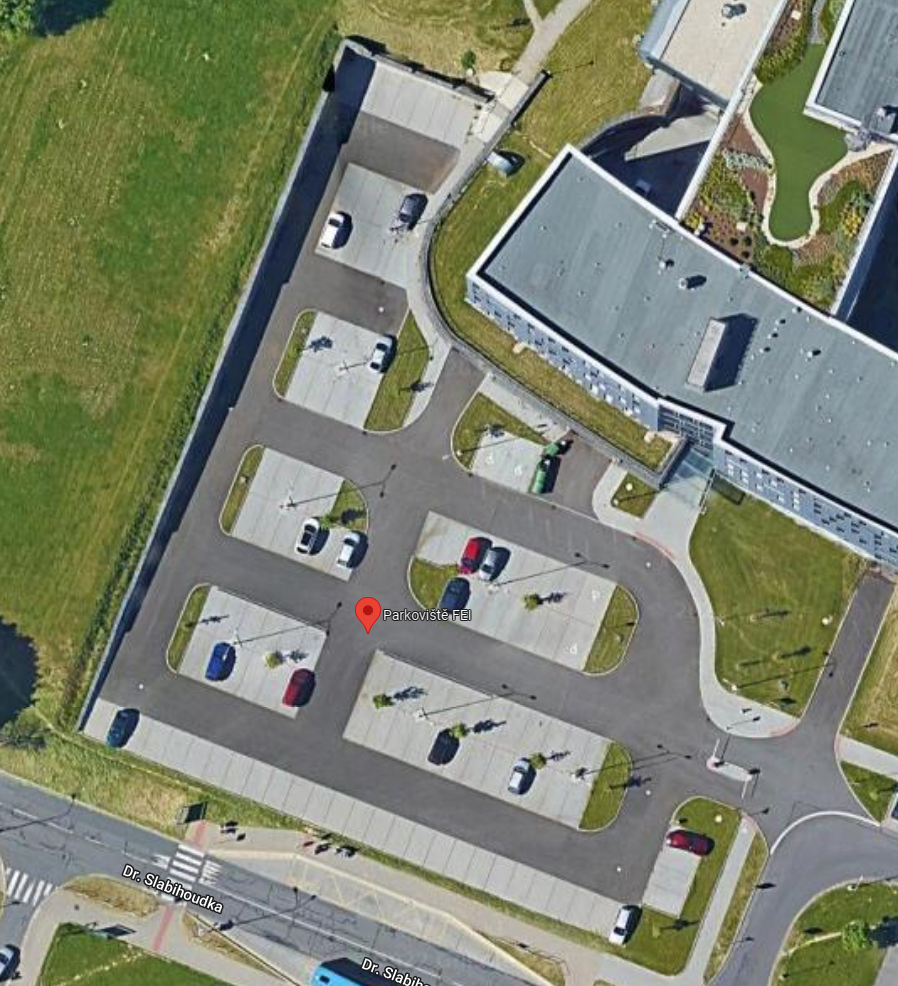
\includegraphics[width=.5\textwidth]{Figures/Mapa.png}   
    \caption{Mapa parkoviště}
    \label{Obr-Navrh-viz}
\end{figure}

Vizualizaci aplikace jsme se rozhodli realizovat v prostředí PROMOTIC. Budou dva účty -- administrátor a uživatel. Administrátor bude mít možnost měnit nastavení svítivosti světel v procentech pro každou hodinu pomocí posuvníků.

V aplikaci (vizualizaci), v našem řešení jsme se rozhodli pro PROMOTIC, existují dva účty. Jeden účet je administrátora, který může měnit nastavení svítivosti světel v procentech pro každou hodinu pomocí posuvníků. V případě, že se zhorší viditelnost, svítivost se dle „závažnosti“ situace procentuálně zvýší. Systém je schopen reagovat téměř okamžitě, záleží tedy na programátorovi, jakou frekvenci vyčítání dat ze senzorů zvolí. Ve druhém účtu je možné pouze sledovat stav, tedy na kolik procent daná lampa svítí. V případě například energetické krize, svátků, je možné světla vypínačem vypnout pro úsporu energie. PROMOTIC není zásadní pro běh aplikace, můžeme využít i jiné vizualizační programy, pokud podporují komunikaci přes UDP protokol (např. LabVIEW). Ukládáme hodnoty senzorů při určování osvětlení, požadovanou intenzitu osvětlení administrátorem, tato data jsou pak sledována právě vizualizací a slouží pro zpětnou kontrolu funkčnosti. 


Jako potencionální chyby řešení můžou být: 
\begin{itemize}
    \item vliv záškodníků na senzory
    \item špatně (nedostatečně) nastavené hodnoty osvětlení ve vizualizaci adminem
    \item delší počáteční ladění systému
\end{itemize}


% \begin{table}[htbp]
% 	\centering
% 	\caption{Definice I/O}
% 	\begin{tabular}{ccccc}
% 		\hline
% 		I/O 
%         & Název proměnné    &Datový typ & Popis \\ \hline
% 		\multirow{3}{*}{I} 
%         & BehLinky          & BOOL      & zapínání/vypínání běhu linky \\
% 		& PaletaVysunuta    & BOOL      & snímač pro vysunutí palety \\ 
% 		& Zrychleni   		& UINT      & volba rychlosti pásu \\ \hline
%         \multirow{6}{*}{O} 
% 		& Snimac            & BOOL      & snímač výrobků \\
% 		& AplikatorFolie    & BOOL      & indikátor aplikátoru folie \\
% 		& HorkovzdusnyFen   & BOOL      & indikátor horkovzdušného fénu \\
% 		& VysouvaciRameno   & BOOL      & indikátor vysouvacího ramena \\
% 		& PocetVyrobku      & UINT      & počítání výrobků \\
% 		& PocetPalet        & UINT      & počítání palet \\ \hline
% 	\end{tabular}
%     \label{Tab-IO}
% \end{table}


\endinput

\chapter{Dokumentace technologie}




\endinput

\chapter{Softwarová analýza}

Bude zapotřebí hlavní program (nepoptřebujující GUI), který bude zpracovávat data získaná ze senzorů a ty pak kontrolovat, zda jsou spravné. Poté přes konfigurační soubor bude periodicky načítat chtěnou hodnotu, kterou porovná s daty ze senzoru a nastaví je na světlech. Mezitím bude periodicky posílat přes UDP protokol data pro vizualizaci (vlastní komunikační protokol, který bude obsahovat, hodnoty konfiguračního souboru, poslední data ze senzorů, boolean podezdření poruchy senzoru a port pro příjem dat k ovládaní přes vizualizaci).

K aplikaci budou mít přístup dva typy lidí -- administrátor a uživatel. Na nejnižší úrovni je uživatel, který může pouze sledovat stavy světel a senzorů. Správce (technik) navíc může vypínat a zapínat celkové osvětlení, upravovat config soubor a manuálně nastavovat intenzitu osvětlení (viz \autoref{Obr-Use_Case_Diagram}). 


Seznam funkcí, které aplikace umí:

\begin{itemize}
    \item sběr procentuálních hodnot osvětlení
    \item sběr viditelnosti ze senzorů
    \item sběr požadovaných procentuálních hodnot skrz vizualizaci
    \item posílaní a následné nastavení chtěné intenzity světla
    \item kontrola senzorů - vždy po sběru dat senzorů
    \item posílaní aktualního stavu vizualizaci
    \item výpočet chtěné intenzity: vezme chtěnou základní hodnotu s configu a upraví ji podle dat získaných senzory 
    \item nastavení config souboru pomocí vizualizace
    \item ukladání dat
    \item kontrola přihlášení od vizualizace.
    \item přepočítaní intenzity (zavolané vizualizací čí změnou config souboru)
\end{itemize}

\section{Komunikace}

Komunikace s osvětlením buď pomocí bezdrátového připojení opět pomocí UDP pravděpodobně.
Jinak připojení ke světlem drátovým vedením.
Komunikace s vizualizací přes UDP

\begin{figure}[H]
    \centering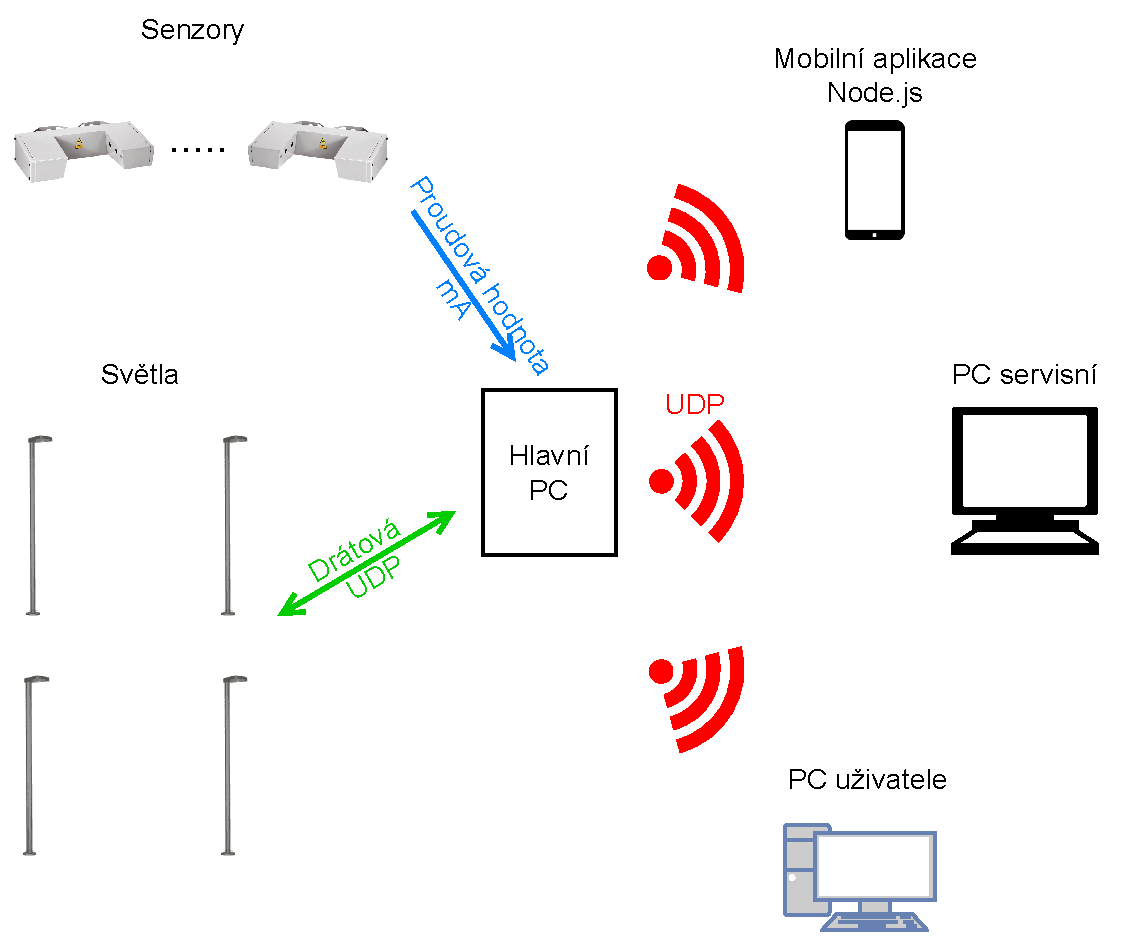
\includegraphics[width=.8\textwidth]{Figures/udp.drawio.pdf}   
    \caption{Komunikace}
    \label{Obr-Komunikace}
\end{figure}

\autoref{Obr-Komunikace} nám popisuje komunikaci našeho řešení pro osvětlení parkoviště. Senzory posílají na hlavní PC analogovou proudovou hodnotu. Pomocí drátového UDP protokolu posílají světla aktuální hodnoty na hlavní PC, který zpětně je schopný přes UDP světla ovládat a nastavovat tedy jejich hodnotu svítivosti. Dále je schopen komunikovat s PC uživatele, který má naší aplikaci vytvořenou v prostředí Promotic, případně se servisním PC, a to bezdrátově (wifi). Dále existuje možnost pomocí Node.js komunikace s mobilním telefonem, kterou momentálně nevyužíváme.



\section{Analýza dokumentů}

\section{Analýza obsahu a struktury informací}

\section{Analýza toku informací}

\section{Analýza slabých míst}


\endinput

\chapter{Systémová specifikace}

\section{Výchozí situace a cíle}

Ovládání světel na parkovišti na základě environmentálních podmínek:
\begin{enumerate}
    \item Pomocí určení základní časové linie
    \item Zesílení intenzity při nízké viditelnosti
    \item Sledování dat ohledně viditelnosti
\end{enumerate}

Ovládání se provádí automaticky, případně se dá vypnout. Při automatickém ovládaní se světlo řídí nahraditelným configem.


\section{Vztah okolí k provozování systému}

Pouze stačí počáteční nastavení, systém následně funguje automaticky. S žádnými daty zvenčí se momentálně nepracuje.
Počet sledujících téměř neomezený, figurují dva účty -- v jednom je umožněno pouze sledování, ve druhém užití se jednou měsíčně nastavují základní svítivosti.


\section{Funkční požadavky} 

\begin{itemize}
    \item funkce pro sběr dat ze senzoru čte hodnoty z připojených senzorů
    \item funkce naslouchače UDP (očekává zpětnou vazbu z vizualizace -- nastavení jendnotlivých světel a nastavení configu)
    \item funkce vysílaní UDP (slouží pro zobrazení vizualizace)
    \item funkce pro nastavení hodnoty na světlech
    \item nastavení config souboru
\end{itemize}

\section{Nefunkční (ostatní) požadavky}

Reakční časy by klidně mohli být i v řádech minut (když se jedná o automatickou funkci), avšak v případě vizualizace a ovládání by čas neměl přesáhnout minutu, především aby uživatel věděl, že je software funkční.
Výpadek nás moc neovlivní -- data by měli být uložené na disku v config souboru, takže při opětovném spuštění je akorát zapotřebí načíst data ze senzoru a denní dobu a pak software pokračuje v předchozí funkci. (světla taky mohou vypadnout, takže proto je potřeba hned načíst čas s daty a poslat nové požadavky)


\section{Uživatelská rozhraní}

Vizualizace je vytvořena v SCADA systému PROMOTIC. PROMOTIC je komplexní SCADA objektový softwarový nástroj pro tvorbu aplikací, které monitorují, řídí a zobrazují technologické procesy v nejrůznějších oblastech průmyslu. Tento systém byl zvolen pro tvorbu vizualizační aplikace z důvodu jednoduchosti vytváření aplikací a dostupnosti. Tento vývojový software je k dispozici jako FREEWARE, tzn. zdarma ke stažení, ale s menším omezením. PROMOTIC obsahuje širokou paletu technologických obrázků, ikon atd. Výhodou je, že lze importovat vlastí obrázky do grafického panelu pro další užití. \parencite{PROMOTIC}

Vizualizace se skládá z mapy svítidel a senzorů na parkovišti, kde se nachází ikony jednotlivých světel a senzorů, jejich označení a aktuální stav světla nebo senzoru dle barvy rozsvícení ikony. Dále se skládá z vizuální reprezentace procentuálního nastavení svítivosti a jeho hodnoty se zobrazují dle aktuálního nastavení v barech pro určitou hodinu dne. Uživatel se automaticky přihlásí po prvotním zapnutí. Pokud je přihlášený uživatel, může jedině sledovat aktuální stav světel a senzorů a konfiguraci procentuálního nastavení svítivosti (viz \autoref{Obr-Viz_uziv}). Pokud je přihlášený administrátor, může manuálně upravovat konfig procentuálního nastavení svítivosti pomocí táhel v reálném čase (viz \autoref{Obr-Viz_admin}). Administrátor může vypínat a zapínat všechny světla najednou pomocí tlačítka. Dále je mu umožněno odhlásit se tlačítkem odhlásit. 


Jednotlivé stavy světel a senzorů:


\includegraphics[width=.04\textwidth]{Figures/zelene.png}
\dots světlo je aktivní


\includegraphics[width=.04\textwidth]{Figures/zlute.png}
\dots upozornění, že světlo pracuje na 100 \%


\includegraphics[width=.04\textwidth]{Figures/cervene.png}
\dots chyba světla (např. není zapojené)


\includegraphics[width=.04\textwidth]{Figures/sede.png}
\dots světlo je manuálně vypnuté (neaktivní) \\



\includegraphics[width=.04\textwidth]{Figures/senzor_zeleny.png}
\dots senzor je aktivní


\includegraphics[width=.04\textwidth]{Figures/senzor_cerveny.png}
\dots chyba senzoru (např. není zapojené nebo došlo k jeho poškození)


\begin{figure}[H]
    \centering\includegraphics[width=\textwidth]{Figures/PROMOTIC_admin_vizualizace.png}   
    \caption{Vizualizace pro administrátora (v plné velikosti viz \hyperref[Sec-Prilohy]{Přílohy})}
    \label{Obr-Viz_admin}
\end{figure}

\begin{figure}[H]
    \centering\includegraphics[width=\textwidth]{Figures/PROMOTIC_uzivatel_vizualizace.png} 
    \caption{Vizualizace pro uživatele (v plné velikosti viz \hyperref[Sec-Prilohy]{Přílohy})}
    \label{Obr-Viz_uziv}
\end{figure}


\section{Chování za chybových situací}

Při sběru dat ze senzoru se vyhodnocuje průměr a v případě odchylky se vyřadí nejvíce odchýlený senzor z průměru a poté se nahlásí jeho chyba. Světla budou pořád svítit na 100 \% (senzor, nebo z důvodu chyby více senzorů, posílá špatné hodnoty) –- tedy i přes den.

\section{Požadavky na dokumentaci}

Vhodné vytvořit manuál popisující vizualizaci a připojení jednotlivých částí systému.

\section{Předávací podmínky}

Možnost softwarového testu, kdy první projde jeden 24-hodinový cyklus v rámci pár minut a následně udělá simulaci snížení viditelnosti. (skvělá ukázka při prodeji).



\endinput

\chapter{UML analýza}



\begin{figure}[H]
    \centering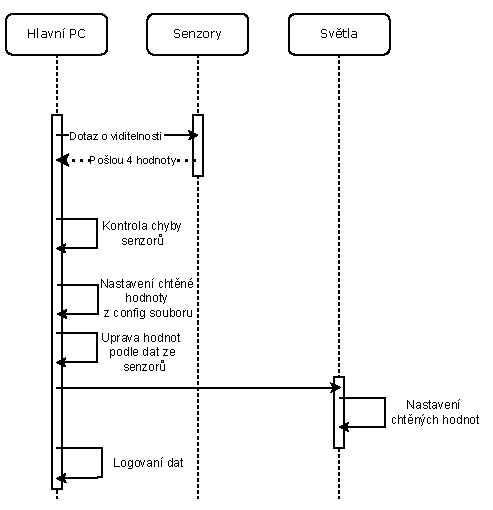
\includegraphics[width=.7\textwidth]{Figures/Sekvencni_diagram.pdf}   
    \caption{Sekvenční diagram nastavení intenzity}
    \label{Obr-Sekvencni_Diagram}
\end{figure}

\begin{figure}[H]
    \centering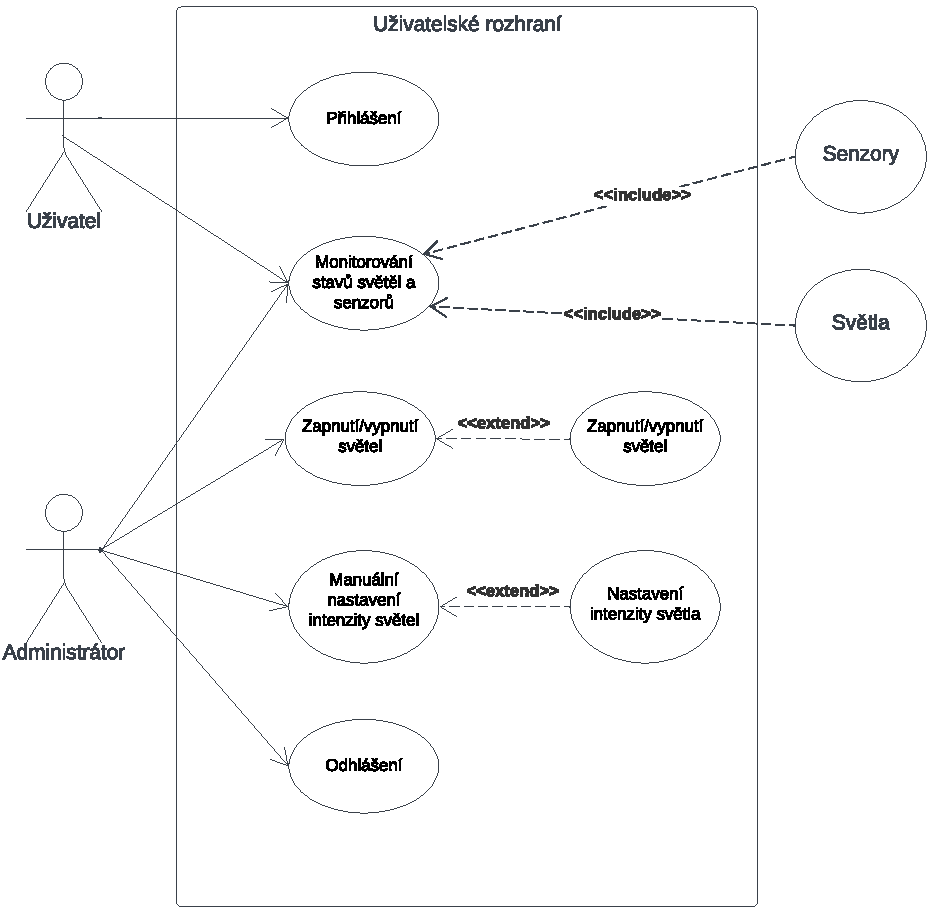
\includegraphics[width=.8\textwidth]{Figures/use_case_diagram_enviro.pdf}   
    \caption{Use Case diagram}
    \label{Obr-Use_Case_Diagram}
\end{figure}

\endinput

\chapter{Závěr}



\endinput

\newpage


% .................................................................... %
% ..................... IMPORT SEZNAMU LITERATURY .................... %

% Seznam literatury
\printbibliography[title={Literatura}, heading=bibintoc]

\chapter{Přílohy}
\label{Sec-Prilohy}

\begin{figure}[ht]
    \centering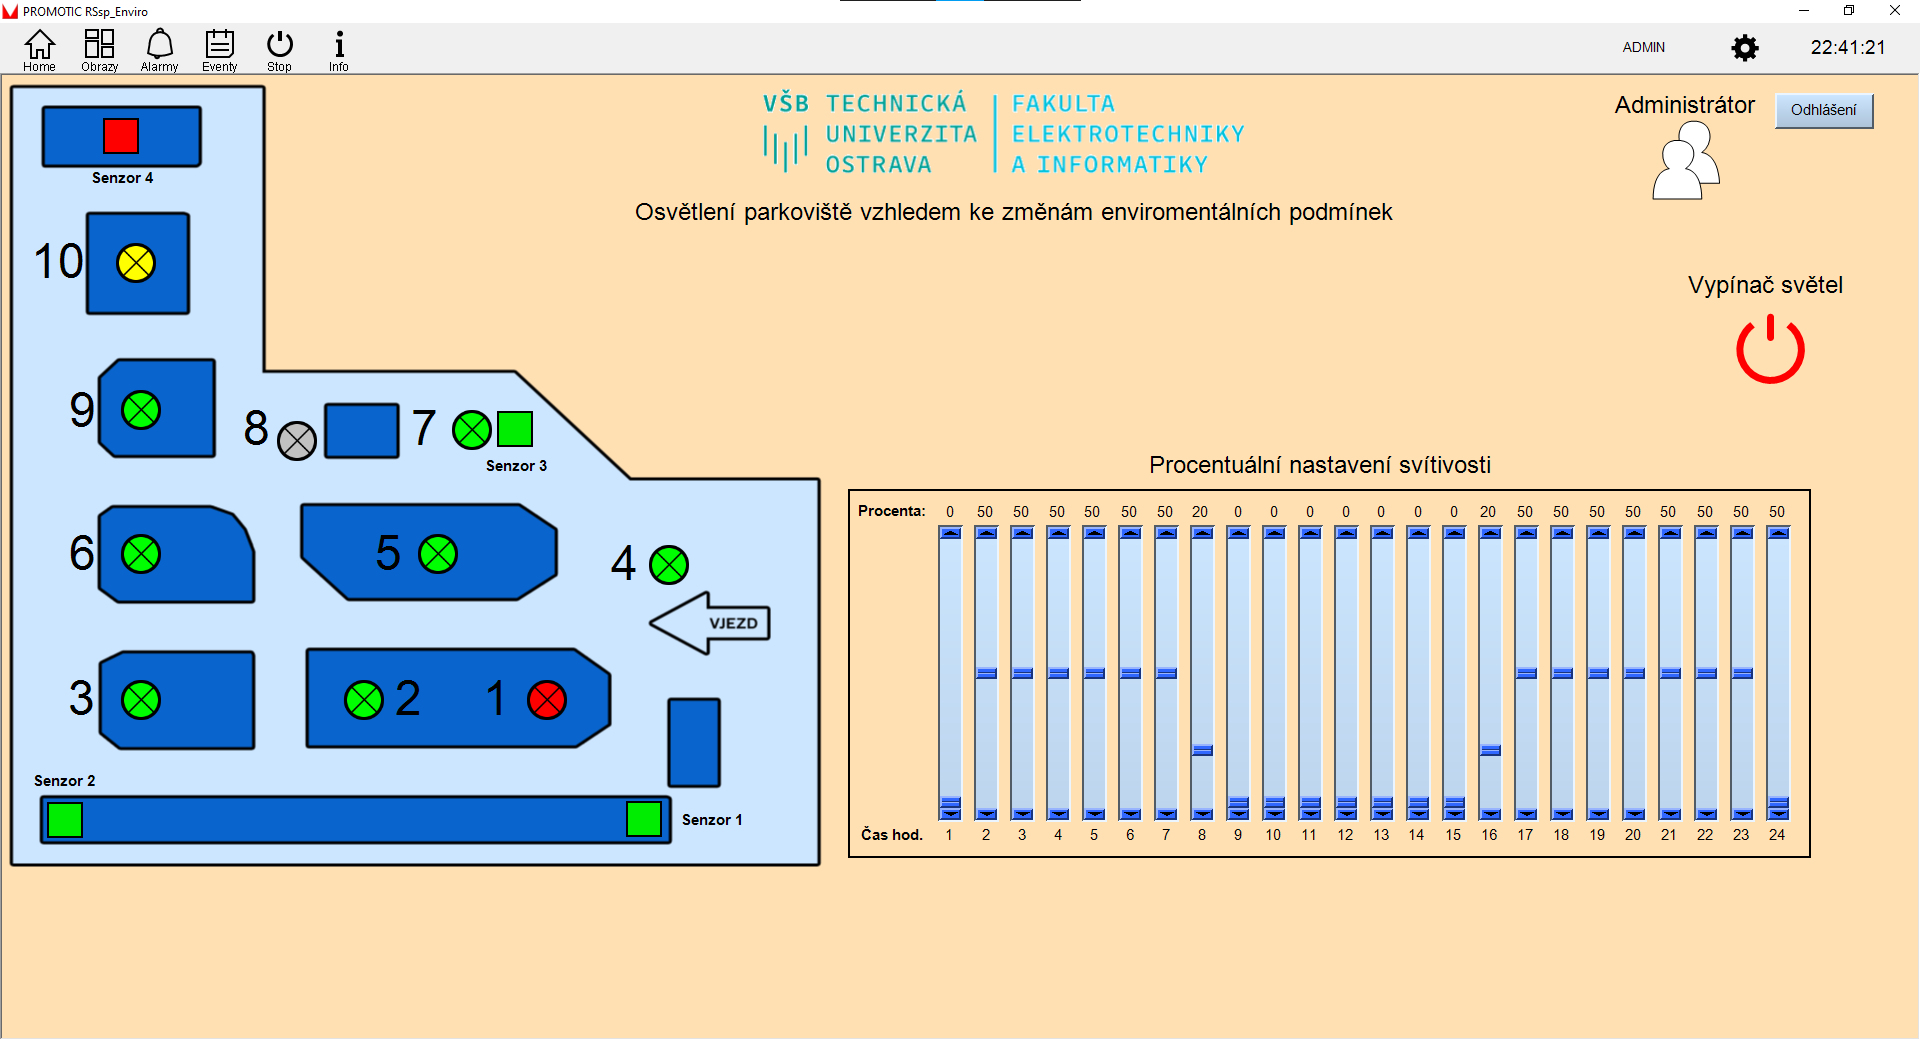
\includegraphics[height=.8\textwidth,angle=-90]{Figures/Promotic_admin_vizualizace.png}   
    \caption{Prvotní návrh vizualizace}
    \label{Obr-Viz_admin-01}
\end{figure}

\begin{figure}[ht]
    \centering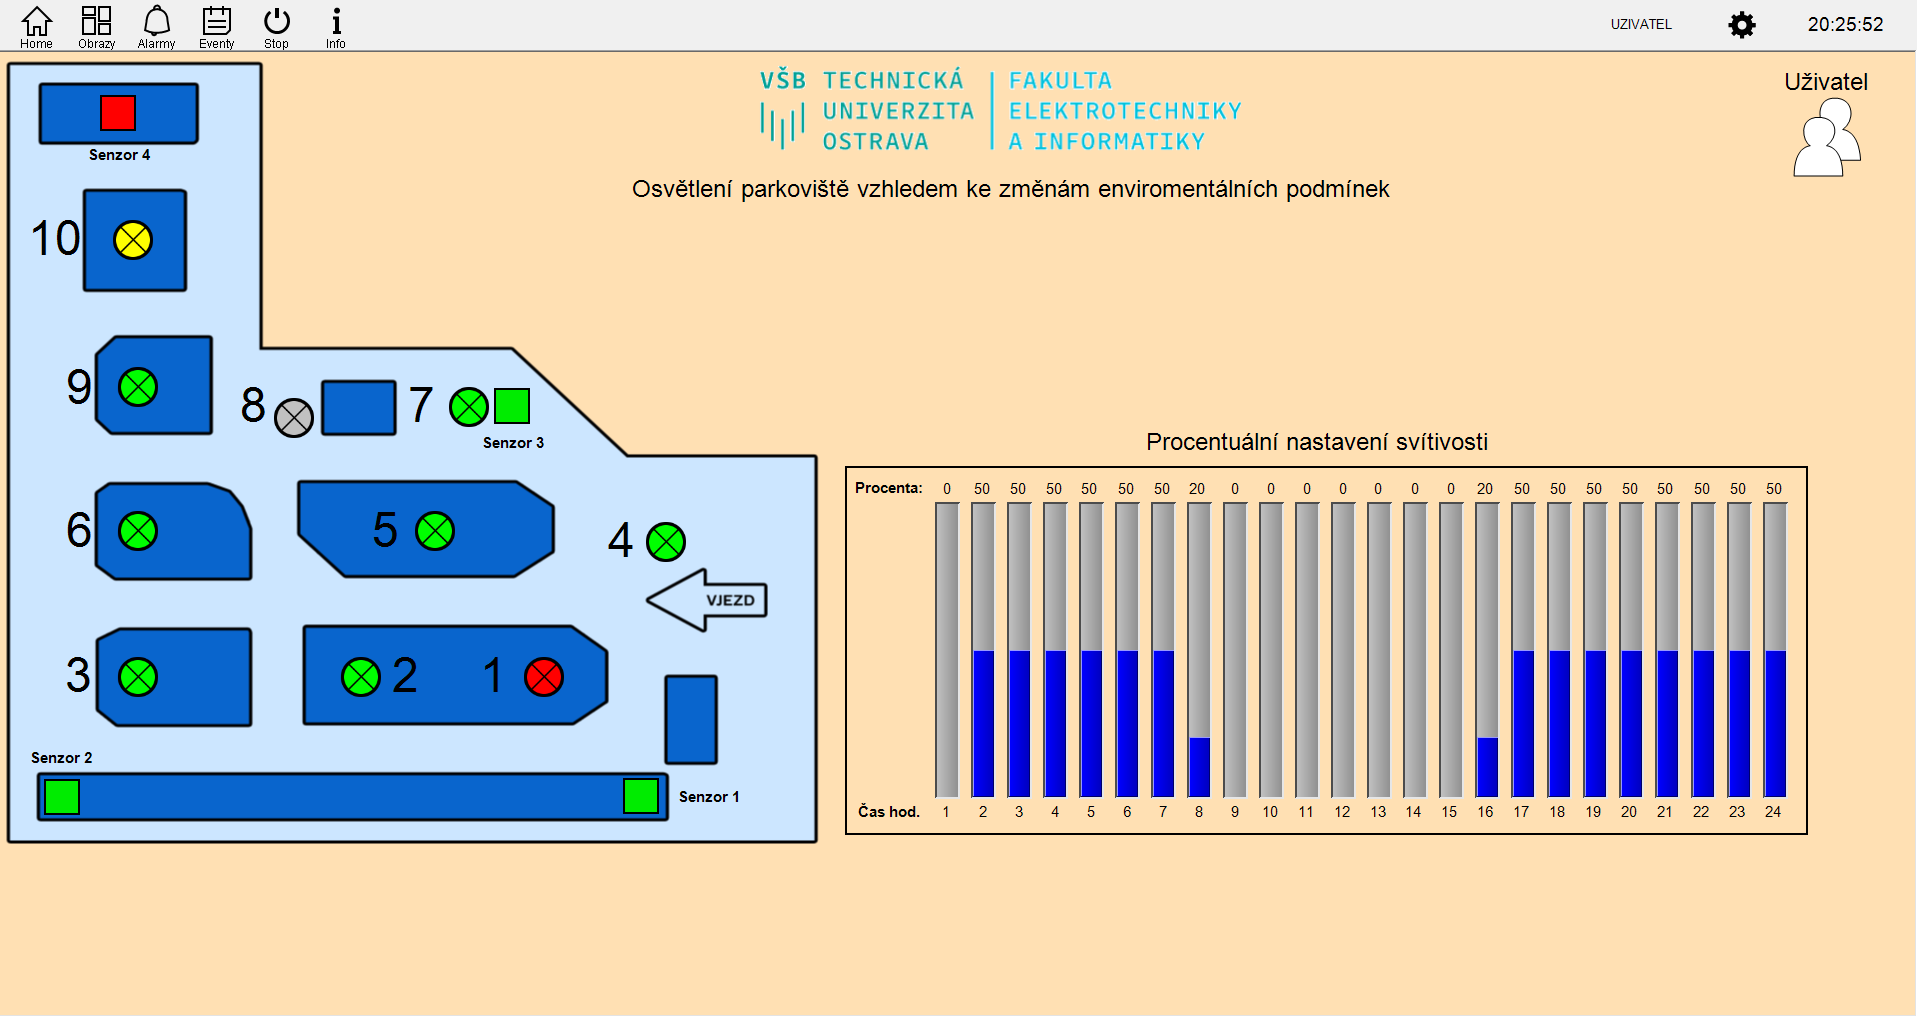
\includegraphics[height=.8\textwidth,angle=-90]{Figures/Promotic_uzivatel_vizualizace.png}   
    \caption{Prvotní návrh vizualizace}
    \label{Obr-Viz_oper-01}
\end{figure}



\endinput

\end{document}
